\tikzstyle{tree}=[draw,circle,fill]
\tikzstyle{every path}=[draw,thick]

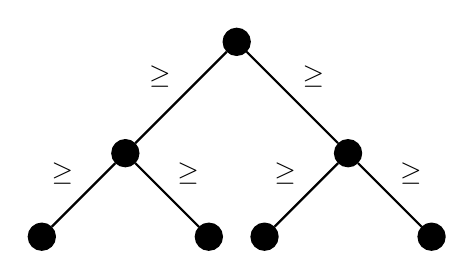
\begin{tikzpicture}

\node[tree] (a) at (0,0) {};

\node[tree,node distance=2cm] (b) [below left of = a] {};
\node[tree,node distance=2cm] (c) [below right of = a] {};

\node[tree,node distance=1.5cm] (d) [below left of = b] {};
\node[tree,node distance=1.5cm] (e) [below right of = b] {};
\node[tree,node distance=1.5cm] (f) [below left of = c] {};
\node[tree,node distance=1.5cm] (g) [below right of = c] {};

\path (a) -- node [above left] {$\geq$} (b);
\path (a) -- node [above right] {$\geq$} (c);

\path (b) -- node [above left] {$\geq$} (d);
\path (b) -- node [above right] {$\geq$} (e);

\path (c) -- node [above left] {$\geq$} (f);
\path (c) -- node [above right] {$\geq$} (g);

\end{tikzpicture}